% Auto-generated LaTeX snippets for CHO manuscript figures.
% Each figure's numerical content traces to experimental_log.md.

\begin{figure}[t]
  \centering
  
\includegraphics[width=0.95\linewidth]{figures/fig_pipeline.pdf}
  \caption{The three-step CHO detection pipeline. Raw electrophysiological signals are first analyzed in the time-frequency domain, where a parametric $1/f$ fit defines bounding boxes around candidate oscillations. Boxes that contain fewer than two complete cycles are rejected to suppress evoked and event-related potentials whose spectral footprint mimics low-frequency oscillations. Surviving boxes are tested against the auto-correlation of the raw signal within each box: the periodicity reported by the positive peaks of the auto-correlation must agree with the center frequency of the box, which rejects harmonic peaks arising from non-sinusoidal waveforms. The output is a set of fundamental oscillations annotated with onset and offset, frequency range, center frequency, and number of cycles.}
  \label{fig:pipeline}
\end{figure}

\begin{figure}[t]
  \centering
  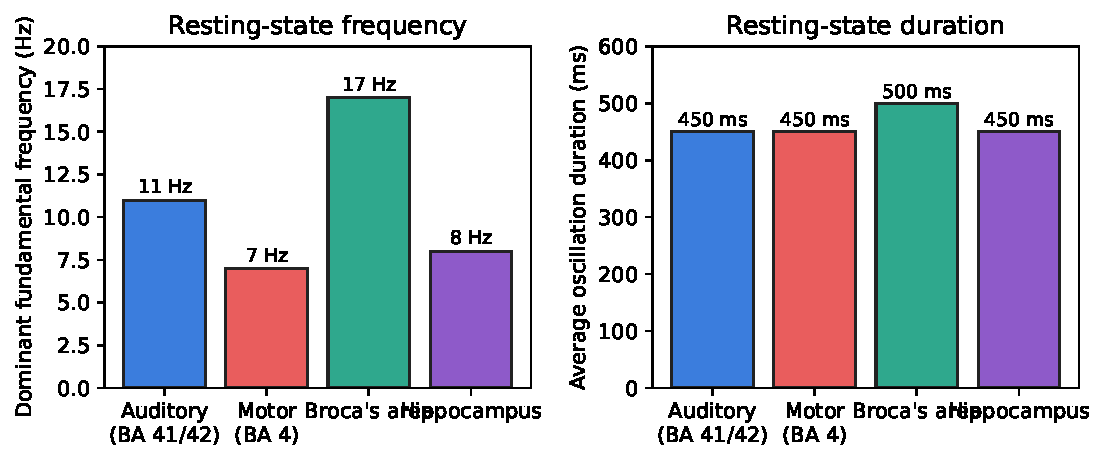
\includegraphics[width=0.95\linewidth]{figures/fig_resting_frequencies.pdf}
  \caption{Predominant fundamental frequency (left) and average oscillation duration (right) detected by CHO across four brain regions during resting state. Primary auditory cortex (Brodmann 41/42) is dominated by 11~Hz oscillations of 450~ms duration; primary motor cortex (Brodmann 4) by 7~Hz oscillations of 450~ms, with additional beta rhythms of $>$500~ms duration (see Figure~\ref{fig:resting}); Broca's area by 17~Hz beta oscillations; and hippocampus by 8~Hz oscillations of 450~ms. Values are taken from CHO applied to SEEG and ECoG recordings at rest.}
  \label{fig:resting}
\end{figure}

\begin{figure}[t]
  \centering
  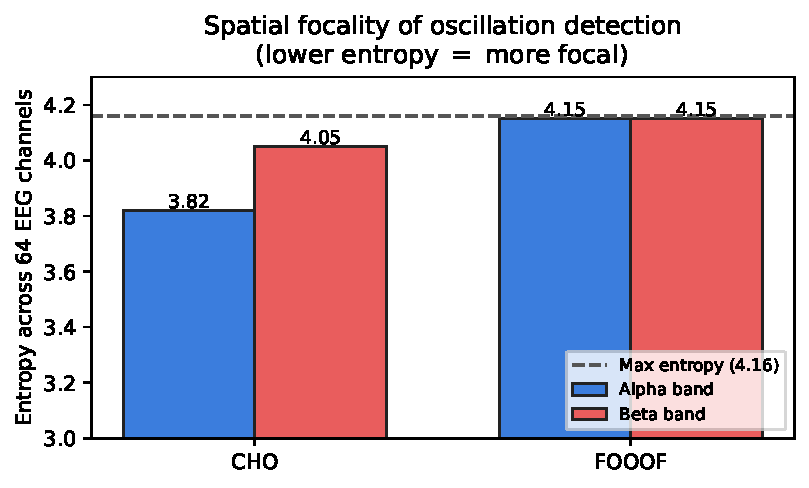
\includegraphics[width=0.85\linewidth]{figures/fig_entropy.pdf}
  \caption{Spatial focality of oscillation detection across 64 EEG channels, quantified by entropy of the per-channel detection distribution. Lower entropy indicates a more focal spatial distribution. The theoretical maximum entropy across 64 channels is $\log_2 64 = 4.16$. In the alpha band, CHO (3.82) produces a substantially more focal distribution than FOOOF (4.15); in the beta band CHO (4.05) is again more focal than FOOOF (4.15). This pattern is consistent with CHO rejecting harmonic peaks that FOOOF detects across spatially diffuse regions.}
  \label{fig:entropy}
\end{figure}

\begin{figure}[t]
  \centering
  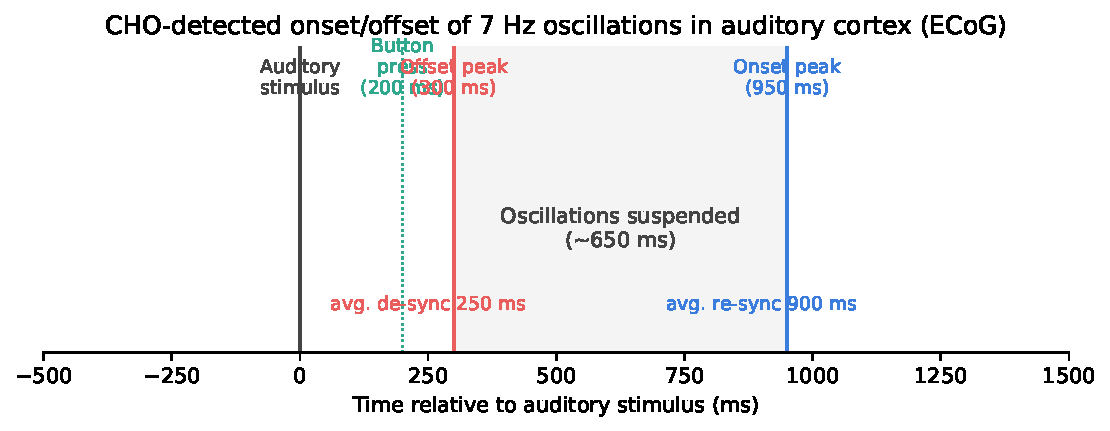
\includegraphics[width=0.95\linewidth]{figures/fig_onset_offset.pdf}
  \caption{Onset and offset of 7~Hz oscillations in auditory cortex during an auditory reaction-time task, detected by CHO from ECoG recordings. After the auditory stimulus, subjects press a button on average at 200~ms post-stimulus. CHO-detected offset of 7~Hz oscillations peaks at 300~ms post-stimulus (i.e., 200~ms post-response), and onset re-emergence peaks at 950~ms post-stimulus. Averaged across subjects, 7~Hz oscillations de-synchronize 250~ms and re-synchronize 900~ms post-stimulus.}
  \label{fig:onset_offset}
\end{figure}
